\section{The Symmetry Breaking Problem}
\label{cap:2}


Symmetry breaking is one of the most extensively studied problems in distributed computing. A symmetric system can be defined as a network in which the vertices or processes are in an equivalent relationship; this means that if the processes run the same code, it is possible to permute the processes without changing the behaviour of the system. One example of a symmetric system would be a ring in which there is no unique identifier for the process \cite{boldi1996symmetry}.  

If we consider the previous example where exists an initial state of symmetry in a ring topology and the processes communicate by message passing, there is an admissible synchronous execution for which the processes will continue in the same initial state. In this case, it is necessary a mechanism to break the symmetry. Otherwise, the system cannot escape from the initial state.
%as shown in \cite{angluin1980local} by Angluin.

The fundamental symmetry breaking problems on graph include the maximal matching, vertex colouring, ruling sets and \textit{MIS}. The last one can be considered as the central topic because all the others can be reduced to it \cite{linial1992locality}. Two problems related to the maximal independent set are studied in the literature; finding the \textit{MIS} of general graphs and listing all the \textit{MISs} for a given graph. The next section provides a formal definition of the maximal independent set and a discussion on the sequential approach versus the distributed approach.

\subsection{Maximal Independent Set}

\theoremstyle{definition}
\begin{definition}

Given an undirected graph $G = (V,E)$, a Maximal Independent Set \textbf{MIS} is a set of vertices $S \subseteq V$ if it satisfied the following properties:   

\begin{enumerate}
  \item the set MIS is an independent set meaning that no two vertices $v,u \in S$ are adjacent,
  \item the set S is maximal, with regard to independence, meaning that for each vertex $v \notin MIS$, there exists a neighbour $u$ of $v$ such that $u \in MIS$.
\end{enumerate}

\end{definition}

Figure \ref{fig:graph1} shows an example of undirected an graph $G$ with 8 vertices and 14 edges. There are two \textit{MIS} in this example, showing that it is possible to find more that one solution for the same instance of $G$. The green nodes are part of the \textit{MIS}, in the first \textit{MIS} the number of nodes is 2 and 4 in the second solution. Note that no common edges exist between green vertices and every vertex that it is not part of the \textit{MIS} have a neighbour in it, satisfying the conditions set out above.
 
\begin{figure}[ht]
\centering
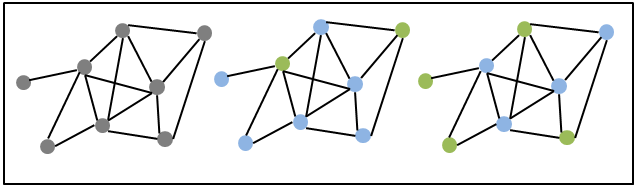
\includegraphics[width=1 \linewidth, height=5cm]{mis-example.PNG} 
\caption{Example of two Maximal Independent Set of a general graph}
\label{fig:graph1}
\end{figure}



The algorithm \ref{algorithm:secuential-mis} describes the general sequential algorithm to find the maximal independent set of a general graph. The time complexity is $O(N)$ since in the worst case, the algorithm has to check every vertex. Another approach to improve this time is desirable. 



\begin{algorithm}
 \caption{Sequential Maximal Independent Set}
 \label{algorithm:secuential-mis} 

\SetAlgoNoLine
\KwResult{MIS Maximal Independent Set}
\KwData{ $G(V,E)$ Graph}
    \While {$V$ is not empty}{
        Choose a vertex $v \in V$
            Add $v$ to the set MIS\;
            Remove from $V$ the vertex $v$ and all its neighbours\;
        }
    
 
\end{algorithm}
 
 
\subsection{Distributed Maximal Independent Set}

This section presents two distributed algorithms to find the \textit{MIS} with the theoretical analysis on time and message complexity. 

The difficulty to find logarithmic lower bound in sequential algorithms motivated the proposal of distributed algorithms.  The approaches to solving problems in distributed computing are deterministic and randomised algorithms.  The use of randomisation is a powerful and efficient technique to solve problems that may take longer time in deterministic algorithms, and it is the preferred method in the literature for symmetry breaking problems.

In 1986, an efficient distributed algorithm was proposed independently by Luby \cite{luby1986simple} and Alon \textit{et al.} \cite{alon1986fast}. Both algorithms are randomised and the expected termination time is $O(log N)$ rounds. It is worth to mention that all algorithms exposed below run in the synchronous model.  

The algorithm\ref{algorithm:luby-mis} describes the original Luby's algorithm. Prove the correctness of this algorithm is very simple. If a process $p_i$ joins the \textit{MIS}, in a round $r$, no other neighbour of $p_i$ join the set in $r$ or in any other $r\prime$. The algorithm at the end produces a \textit{MIS} because the processes with the highest degree will decide to enter the \textit{MIS} in each round until all processes become inactive.

\begin{definition}

An algorithm terminates with high probability (w.h.p.) within $O(t)$ time if it does so with probability at least $1-\frac{1}{n^c}$ for any choice of $c\geq 1$.

\end{definition}

% \theoremstyle{theorem}
\begin{theorem}

Algorithm \ref{algorithm:luby-mis} computes a maximal independent set for any graph  in $O(\log n)$  rounds with high probability.

\end{theorem}


\begin{algorithm}
 \caption{Luby's Algorithm, code for each process $p_i$ $i = 1$ to $N$}
 \label{algorithm:luby-mis} 

\SetAlgoNoLine
\KwResult{MIS Maximal Independent Set}
\KwData{ $G(V,E)$ Graph}
    \While {V is not empty}{
        Choose a random set of vertices $S ⊆ V$, by selecting each vertex $v$ independently with probability $1/(2d(v))$, where d is the degree of $v$\;
        For every edge $e \in E$, if both its endpoints are in the random set $S$, then remove from $S$ the endpoint whose degree is lower. Break ties arbitrarily, e.g. using a lexicographic order on the vertex names\;
        Add the set $S$ to $MIS$\;
        Remove from $V$ the set $S$ and all the neighbours of vertices in $S$\;
        }
\end{algorithm} 


The algorithm \ref{algorithm:main-mis} is a variation of the previous algorithm, and it was proposed by Yves \cite{yves2009optimal}. For this algorithm, in each phase, the half of the edges are removed in expectation. The rounds are split into 2 phases, in each phase, $p_i$ chooses a random value, send it to its neighbours and wait to receive the value from all its neighbours. If the process has the minimum value, then it joins the \textit{MIS}. In the second phase, if $p_i$ decided to join the \textit{MIS}, then $p_i$ notified to its neighbours that it is part of the \textit{MIS}. If $p_j$ receives the last notification message from $p_i$, then $p_j$ decide not to join the \textit{MIS}. At the end of this phase, every process that decided against joining or not the \textit{MIS} become inactive for the next rounds.


\begin{algorithm}
 \caption{MIS Algorithm, code for each process $p_i$ from $i = 1$ to $N$}
 \label{algorithm:main-mis} 

\SetAlgoNoLine
\KwResult{MIS Maximal Independent Set}
\KwData{ $G(V,E)$ Graph}
    \While {V is not empty}{
        $p_i$ select a random number $r(v)$ between [0,1] and sends to its neighbours\;
        If $r(v) < r(w)$ for all neighbours $w \in N(v)$ of $p_i$, remove myself from $V$ and enter to the MIS \newline
        Inform my neighbours that I am a MIS member and terminate\;
        If $p_i$ heard that my neighbour $p_j$ is in the MIS, remove myself from the $V$ and terminate\;
        }
\end{algorithm}

% Lemma 7.14 (Edge Removal). In a single phase, we remove at least half of
% the edges in expectation.

The correctness is very intuitive and similar to the Luby's algorithm. In each phase, one process $p_i$ joins the \textit{MIS} only if it has the smallest value among its neighbours. At the end of the phase, the entire $p_i$ neighbourhood become inactive (including $p_i$) and all processes terminate the local algorithm. The result is that there are no two processes that share the same link in the MIS. This set is maximal because at least one vertex (with the global smallest value) will enter into the \textit{MIS} per round. Hence there is a progression in each round. If at some round, a vertex has no neighbours, it automatically joins the set and become inactive. This sequence continues in the following rounds until every process becomes inactive.



% \theoremstyle{theorem}
\begin{theorem}

Algorithm \ref{algorithm:main-mis} computes a maximal independent set for any graph in $O(\log n)$ rounds with high probability.

\end{theorem}

 When a vertex $v$ joins the \textit{MIS}, all its edges are removed from $E$ but also all edges of any neighbour of $v$. In general, this number is much greater than the degree of $v$. So there is a high probability that the topology decreases very fast. Indeed, this is the mechanism to demonstrate the lower bound of $O(\log N)$.  In the section \ref{chap:6} (Evaluation of results), this supposition is tested experimentally calculating the diameter of the remaining part of the active network. 
 
 
Message complexity depends on the number of edges of the graphs for both algorithms. In each round $p_i$ send messages to each neighbour, so at least two messages are sent per edge, one in each direction. Note that the number of vertices in each round decrease progressively and so does the number of edges. The message complexity of the algorithms is $O(m)$, being m the number of process in the topology \cite{luby1986simple}.


 Until now, these two algorithms are faster than the best deterministic algorithms for general graphs. There have been some improvements but not for general graphs. For instance, Panconesi \textit{et al.} \cite{panconesi1996complexity} proposed a $O(\Delta + log^* N)$ algorithm for specific graphs with bounded degree, however, the original algorithms are still faster when the running time is expressed as a function of $N$ and for any type of graph.
 

 

% . This algorithm operates in synchronous rounds. In line 2, every process select a random number to in order to break the symmetry with its neighbours, line 3 makes sure that if a vertex v join the MIS, no other neighbour of v join the MIS at the same time, this is true because the execution  occurs in rounds. the line 4 makes sure that any vertex that has a neighbour in the MIS, join the MIS at any point. 
